\section{Appendix: Use Case Scenario}

\subsection{Motivation}
This appendix describes recent UX research within the context of the NDN (Named Data Networking) project. The UX design has primarily been focused on a mobile fitness application. The broad goal of the fitness app is to develop a non-trivial application to test the NDN network architecture. As an extension of these layered goals, the UX design process has been focused on both the mobile fitness application, the management of personal data (id manager), and the process of joining the NDN internet. The UX research/design has primarily taken the form of speculative concept sketches, user narratives and scenarios, to help think through possible futures involving the NDN internet. Within the context of the NDN project the hope is that UX design can function as an entry point for discussing critical "values in design" issues surrounding security and identity. 

Consider non-technical knowledge of computing and the internet. A large percentage of internet users don't know what an internet browser is, with the difference between their operating system or "desktop" and the browser being fuzzy at best. By extension, understandings of domains and urls are limited, to marketing campaigns from the first .com boom. Many younger internet users have little concept of an internet outside of their popular social platforms. At the same time the concept of an "app" has become widely known. In the most simple, and almost mystic of ways, the app has become a magical button that offers services of amusement or utility. While the app has its internal functionality, the ontological foundation of the user experience of the "app" is the on/off, in/out experience of the phone. This "in/out" experience reproduces a silo like concept of the application as a discrete thing, something you put in your pocket, rather than a series of interrelated systems. 

For the NDN internet user, the interoperability of structured data, will translate into a user experience that reorients the popular understanding of apps and urls. With this shift will be a greater awareness of how one's apps and devices are speaking to each other. The on/off quality of the discrete app will be replaced with an and/or, intuitively modular, way of understanding applications and the flow of data and systems.
  
\begin{figure*}
\begin{center}
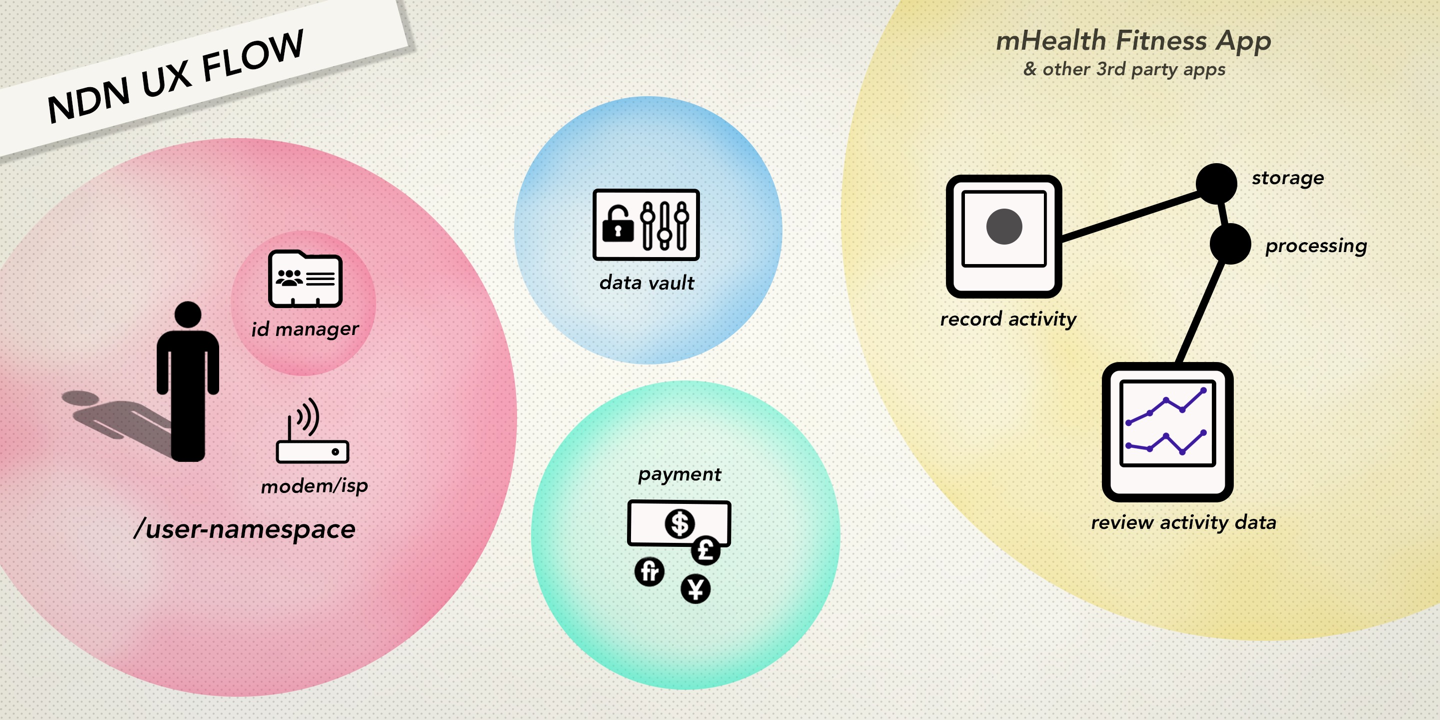
\includegraphics[width=.5\textwidth]{figures/ux-scenario}
\caption{This sketch illustrates the user's spheres of experience and the conceptual-emotional proximity of how systems relate to one another from the user's perspective. Data is stored, published, and managed, by the data vault. Intimate to the user's navigation of third party applications is the "id manager" which gives the user a fast and easy way to specify which identities to use with specific applications. Third party applications exchange structured data within a data-dissemination based paradigm, giving users greater access to a modular understanding of systems.}
\label{fig:uxsketch}
\end{center}
\end{figure*}

\subsection{Steps in Application Use} 

\paragraph*{1. User Joins the NDN Network.} 
The user unpacks their new modem. On their computer/device the user runs an application from the internet provider that walks them through process of connecting to the NDN internet. The user gets connectivity to the NDN Internet. The application then walks the user through the process of claiming a namespace and authenticating connections with personal devices. 
   
\paragraph*{2. Signs Up for Personal Data Vault / Identity Manager.}

(This could happen as part of application signup.)

Once the user has finished claiming a name space and connecting devices, the application presents the user with a menu of recommended "personal data guardians" or data vaults. As a professional service provider the data guardian functions as a confidant for archiving and managing self generated personal data. The data vault provides the user with automated data management, granular data preferences, and programatic controls. While the data vault is technically a separate application from the identity manager, from the user's perspective they are closely connected. The identity manager allows fast on-the-go authentication and data management. 

The user selects a data vault that comes with technical and legal support in the event of a problem, and a collection of additional identity management and data visualization applications for specific aspects of the user's life. The user is taken through a process of selecting key preferences, and authenticating a connection with their various devices. Devices have default data exchange preferences, with brief explanations of what they are. 

The user is given a simple faceted search tool to narrow their focus to data types, specific data exchanges, devices, and 3rd party client applications. While the user can edit the preferences of a single exchange, the user can also create programmatic changes, that effect all data exchanges or certain data types. 
\begin{itemize}
\item Preferences for local device exchanges. 
\item Preferences for device to manufacture exchanges. 
\item Preferences for new applications? 
\end{itemize}
This raises several issues for us to consider:
\begin{itemize}
\item How does the user know that they are actually talking to the right PDV?   
\item How does the user know what data belongs to what? 
\item What does the confirmation of a secure connection look and feel like across devices? 
\end{itemize}

\paragraph*{2b. Payment.}
 Once complete the user submits their payment information.    
 Bitcoin, Apple Pay, payment specific devices and objects, etc... 
     
\paragraph*{3. Identity Manager.}
Once signed into the Identity Manager, the user can see a summary of the various data exchanges they have. The authentication process, or signing in process, will in many cases be through some form of biometrics, finger print, voice, etc. But there will have to be an option for those that refuse biometrics. As mentioned above, the identity manager allows fast on-the-go authentication and data management through a high-level notion of "identities" that have associated preferences. An identity is about which apps speak to each other, and how they speak to each other. 

\paragraph*{4. Fitness Application.}  
The user downloads/bookmarks the fitness application. Confirmation of authentic connection. 
When initially launching the application, the ID manager gives the user options for which "identity" to associate with the application (when and where). The personal data vault request permissions to provide the application with location (etc) data, with associated default preferences, with recommendation for how the data should be formatted/summarized/edited before sharing. Highlights from the default preferences include opting to contribute anonymized data to California State Park user research effort and sharing data with fitness data visualization app / fitness with friends app. While the fitness activity recorder and fitness visualization apps are branded under a single California State Park identity and UX experience, they function as separate applications, one publishing data for the other. The user begins using fitness application. After running or walking a complete loop around the park a short audio clip is pushed to the user. The audio clip gives the user a short historic piece of information about the park and surrounding area. For every loop the user is give a short audio piece. 

\paragraph*{4b. Payment.}

\paragraph*{5. Fitness Visualization \& Fitness with Friends App .}
The user goes to the visualization app and explores their fitness data through various visualization tools.      

\paragraph*{6. Content push} 

Location-based content push

\paragraph*{7. Identity Manager.} 
Returning to the ID Manager, the user can now see their fitness applications preferences have been added.  A friend sends the user an invitation to join their "Fitness with Friends Group," which the user accepts, linking their fitness data to the application. The ID manager, asks the user if they would like to send the fitness with friends app a statistically averaged (or "edited") version of their data.    
Third Party Applications? Flow between devices / vault / client app? 

\paragraph*{8. Usage...} 

\paragraph*{N. Exiting Process.}
How to exit?
\begin{itemize}
\item Exit from third party online systems? 
\item Exit from the data vault? 
\item Exit from data manager? 
\item Exit from the name space? 
\end{itemize}

\subsection{User scenarios}

\subsubsection{Anna \& the Salon}
Anna lives in east Hollywood, and runs a small hair salon in Silver Lake. At home Anna signs up for a name space and personal data vault / manager. At work, Anna's partner Karen signs her up as a co-owner of a data vault / manager for their salon. Data that is specific to Anna and Karen synchronizes across their shared data vault, and their individual fault.  

Karen eventually decides to sell her share of the salon to Anna, and in doing so, signs over complete ownership to the data vault to Anna. Some time later, Anna decides to sell the salon. As part of the sale, an edited version of the data vault / manager is transferred to the new owner. 

\subsubsection{Mark's Fitness}
Mark lives in Lincoln Heights, and regularly goes to the Los Angeles State Historic Park to run around the park track. Mark downloads the fitness application, and starts using it in the park. While running Mark befriends Sarah who also runs in the park. After seeing each other several times, the two exchange contact information, and begin comparing running data. The two use different fitness tracking apps, but use a common app for sharing and comparing their running data. 

Since Mark is using the LASHP fitness app, every time he completes a lap around the park, he receives a short audio piece about Los Angeles History. Knowing his father enjoys LA history and needs to get out more often, Mark shares the audio piece with his father, and  invites him to come along for a walk in the park. Wanting the historic information, Mark's father downloads the fitness app, and starts walking with his son on a weekly basis. 

Because Mark and his father are using the LASHP fitness app, and agreed to the default settings, they are contributing an anonymized version of their data to LASHP for research purposes. After visiting the park regularly for two months, LASHP forwards them a request to fill out a short survey. Mark fills out the survey, and when finished is asked if he wants to invite any of his running partners to contribute to LASHP research. He decides to forward the invitation to Sarah. Sarah receives the invitation, but instead of having to download the LASHP fitness app, she is able to authorize a data exchange with one click, giving LASHP access to an anonymized version of her data. 

\subsection{Open questions}
\begin{itemize}
\item How do users join the NDN network (for the first time, or on the go as a mobile guest)? 
\item How do users understand and manage their data and online identities? 
\item How are encryption keys managed, and/ how is "authentication" understood by users?
What is the user experience of the fitness application? 

\item How can the user experience of the fitness application be emblematic of the data-dissemination paradigm? 

\end{itemize} 


